
\chapter{Desenvolvimento da Aplicação}

O desenvolvimento do protótipo neste trabalho busca ser opção para substituir o software Editor UAL, que é utilizado na UDESC/CEPLAN atualmente. Esse protótipo deve ser prático, atual, acessível e com o código disponível para que possa ser mantido e ampliado. Essencialmente a aplicação foi desenvolvida em linguagens Web, o JavaScript sendo a linguagem de programação, HTML como linguagem de marcação e CSS como estilização. A pesquisa de tradutores foi realizado,  baseado em \citeonline{esmin1998}, um esboço do funcionamento pretendido (Figura \ref{fig:tradutor}), para a simulação dos algoritmos no protótipo proposto.

%Nesse protótipo buscou-se eliminar algumas deficiências básica que existem em ferramentas similares, por exemplo funcionalidade de desfazer durante a edição, pois essas podem fazer com que o seu uso seja desgastante e desanimador. Como mencionado nas limitações a inclusão de funcionalidades que poderiam estar disponíveis ficarão como sugestões, algumas delas são encontradas por exemplo em Ambientes Integrados de Programação, comumente utilizada em outras linguagens.

\begin{figure}[h]
  \caption{Tradutor proposto}\label{fig:tradutor}
  \centering
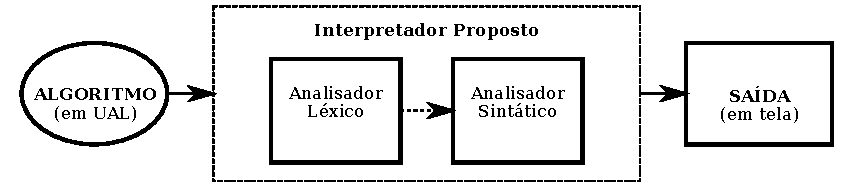
\includegraphics[width=.9\textwidth,height=10cm,keepaspectratio]{figures/interpretador-proposto.pdf}
  \caption*{\footnotesize Fonte: Produção do autor, 2016.}
\end{figure}

%Há caso em que a ferramenta inicialmente utilizada, como o Editor UAL, não é capaz de executar alguns algoritmos mais avançados, levando a necessidade do uso de outro software na mesma disciplina até com possivelmente uma nova linguagem (por exemplo a linguagem de programação C ou C++). Devido a está necessidade alguns educadores optam por usar única linguagem linguagem (C) e algum software, por exemplo Dev C++.

%Inclusive há caso em que a ferramenta inicialmente utilizada não é capaz de executar alguns algoritmos mais avançados. E isto leva a necessidade do uso de outro software na mesma disciplina até com possivelmente uma nova linguagem (por exemplo a linguagem de programação C ou C++), devido a está necessidade alguns educadores optam por esta sendo a única ferramenta utilizada, ignorando linguagem Portugol. Espera-se que diferente o UAL essa limitação possa realmente ser concluída em trabalho futuros, conforme proposto nas conclusões.

\section{Engenharia de Requisitos}

% NOTE Seguindo o modelo de \citeonline{silva2013} de um AVA

No desenvolvimento de software antes de iniciar a codificação, algumas etapas são esperadas e recomendadas para maior assertividade (qualidade, orçamento, prazos). Como explicado por \citeonline{sommerville2011}, neste processo são acordados e especificados os detalhes que satisfazem os envolvidos. Há dois níveis de detalhamento dessa especificação, um para clientes e usuários outro aos desenvolvedores, alto nível e abrangente respectivamente. Análise de requisitos prioriza e classifica os pontos que a aplicação pretende solucionar.

Os \textbf{Requisitos Funcionais} descrevem o que o sistema deve fazer, normalmente são descritos de modo abstrato para a fácil compreensão por seus usuários \cite{sommerville2011}. Puderam para o software ser levantados os requisitos funcionais vistos na Tabela \ref{tab:rf}.

\begin{table}[h]
\centering
  \caption{Requisitos Funcionais}\label{tab:rf}
\begin{tabular}{ c | l }\hline
\textbf{Código} & \textbf{Descrição} \\ \hline
$[$RF001$]$ & Permitir ao aluno edição de código \\ \hline
$[$RF002$]$ & Permitir ao aluno abrir arquivos de texto \\ \hline
$[$RF003$]$ & Permitir salvar o arquivo alterado \\ \hline
$[$RF004$]$ & Permitir visualizar a simulação do programa \\ \hline
\end{tabular}
  \caption*{\footnotesize Fonte: Produção do autor, 2016.}
\end{table}

Já os \textbf{Requisitos Não Funcionais} segundo \citeonline{sommerville2011}, são relacionados não diretamente as funcionalidades, oferecidas pelo sistema aos usuários. O autor também descreve estes requisitos sendo: confiabilidade, desempenho, proteção ou disponibilidade. Foram definidos para o software os requisitos não funcionais presentes na Tabela \ref{tab:rnf}.

\begin{table}[h]
\centering
  \caption{Requisitos Não Funcionais}\label{tab:rnf}
\begin{tabular}{ c | l }\hline
\textbf{Código} & \textbf{Descrição} \\ \hline
$[$RNF001$]$ & O programa deve prezar pelo menor tamanho possível nos arquivos \\ \hline
$[$RNF002$]$ & O sistema deverá rodar em navegador (\textit{browser}) moderno \\ \hline
$[$RNF003$]$ & Deverá ter interface minimalista, mas visualmente agradável \\ \hline
$[$RNF004$]$ & Ser acessível mesmo que desconectado da internet \\ \hline
\end{tabular}
  \caption*{\footnotesize Fonte: Produção do autor, 2016.}
\end{table}

\section{Diagramas UML}

Na etapa de \textbf{Projeto Lógico} tem-se a elaboração de documentos do projeto, fase importante para melhor entendimento do sistema em desenvolvimento. Inclui-se nas seguintes subseções os diagramas UML, foi desenvolvido os diagramas de casos de uso e componentes.

%\begin{center}
%\begin{longtable}{|l|l|l|}
%\caption[Feasible triples for a highly variable Grid]{Feasible triples for
%highly variable Grid, MLMMH.} \label{grid_mlmmh} \\
%
%\hline \multicolumn{1}{|c|}{\textbf{Time (s)}} & \multicolumn{1}{c|}{\textbf{Triple chosen}} & \multicolumn{1}{c|}{\textbf{Other feasible triples}} \\ \hline
%\endfirsthead
%
%\multicolumn{3}{c}%
%{{\bfseries \tablename\ \thetable{} -- continuação}} \\
%\hline \multicolumn{1}{|c|}{\textbf{Time (s)}} &
%\multicolumn{1}{c|}{\textbf{Triple chosen}} &
%\multicolumn{1}{c|}{\textbf{Other feasible triples}} \\ \hline
%\endhead
%
%\hline \multicolumn{3}{|r|}{{(continua)}} \\ \hline
%\endfoot
%
%\hline \hline
%\endlastfoot
%
%0 & (1, 11, 13725) & (1, 12, 10980), (1, 13, 8235), (2, 2, 0), (3, 1, 0) \\
%2745 & (1, 12, 10980) & (1, 13, 8235), (2, 2, 0), (2, 3, 0), (3, 1, 0) \\
%5490 & (1, 12, 13725) & (2, 2, 2745), (2, 3, 0), (3, 1, 0) \\
%8235 & (1, 12, 16470) & (1, 13, 13725), (2, 2, 2745), (2, 3, 0), (3, 1, 0) \\
%10980 & (1, 12, 16470) & (1, 13, 13725), (2, 2, 2745), (2, 3, 0), (3, 1, 0) \\
%13725 & (1, 12, 16470) & (1, 13, 13725), (2, 2, 2745), (2, 3, 0), (3, 1, 0) \\
%16470 & (1, 13, 16470) & (2, 2, 2745), (2, 3, 0), (3, 1, 0) \\
%19215 & (1, 12, 16470) & (1, 13, 13725), (2, 2, 2745), (2, 3, 0), (3, 1, 0) \\
%21960 & (1, 12, 16470) & (1, 13, 13725), (2, 2, 2745), (2, 3, 0), (3, 1, 0) \\
%24705 & (1, 12, 16470) & (1, 13, 13725), (2, 2, 2745), (2, 3, 0), (3, 1, 0) \\
%27450 & (1, 12, 16470) & (1, 13, 13725), (2, 2, 2745), (2, 3, 0), (3, 1, 0) \\
%30195 & (2, 2, 2745) & (2, 3, 0), (3, 1, 0) \\
%32940 & (1, 13, 16470) & (2, 2, 2745), (2, 3, 0), (3, 1, 0) \\
%35685 & (1, 13, 13725) & (2, 2, 2745), (2, 3, 0), (3, 1, 0) \\
%38430 & (1, 13, 10980) & (2, 2, 2745), (2, 3, 0), (3, 1, 0) \\
%41175 & (1, 12, 13725) & (1, 13, 10980), (2, 2, 2745), (2, 3, 0), (3, 1, 0) \\
%43920 & (1, 13, 10980) & (2, 2, 2745), (2, 3, 0), (3, 1, 0) \\
%46665 & (2, 2, 2745) & (2, 3, 0), (3, 1, 0) \\
%49410 & (2, 2, 2745) & (2, 3, 0), (3, 1, 0) \\
%52155 & (1, 12, 16470) & (1, 13, 13725), (2, 2, 2745), (2, 3, 0), (3, 1, 0) \\
%54900 & (1, 13, 13725) & (2, 2, 2745), (2, 3, 0), (3, 1, 0) \\
%57645 & (1, 13, 13725) & (2, 2, 2745), (2, 3, 0), (3, 1, 0) \\
%60390 & (1, 12, 13725) & (2, 2, 2745), (2, 3, 0), (3, 1, 0) \\
%63135 & (1, 13, 16470) & (2, 2, 2745), (2, 3, 0), (3, 1, 0) \\
%65880 & (1, 13, 16470) & (2, 2, 2745), (2, 3, 0), (3, 1, 0) \\
%68625 & (2, 2, 2745) & (2, 3, 0), (3, 1, 0) \\
%71370 & (1, 13, 13725) & (2, 2, 2745), (2, 3, 0), (3, 1, 0) \\
%74115 & (1, 12, 13725) & (2, 2, 2745), (2, 3, 0), (3, 1, 0) \\
%76860 & (1, 13, 13725) & (2, 2, 2745), (2, 3, 0), (3, 1, 0) \\
%79605 & (1, 13, 13725) & (2, 2, 2745), (2, 3, 0), (3, 1, 0) \\
%82350 & (1, 12, 13725) & (2, 2, 2745), (2, 3, 0), (3, 1, 0) \\
%85095 & (1, 12, 13725) & (1, 13, 10980), (2, 2, 2745), (2, 3, 0), (3, 1, 0) \\
%87840 & (1, 13, 16470) & (2, 2, 2745), (2, 3, 0), (3, 1, 0) \\
%90585 & (1, 13, 16470) & (2, 2, 2745), (2, 3, 0), (3, 1, 0) \\
%93330 & (1, 13, 13725) & (2, 2, 2745), (2, 3, 0), (3, 1, 0) \\
%96075 & (1, 13, 16470) & (2, 2, 2745), (2, 3, 0), (3, 1, 0) \\
%98820 & (1, 13, 16470) & (2, 2, 2745), (2, 3, 0), (3, 1, 0) \\
%101565 & (1, 13, 13725) & (2, 2, 2745), (2, 3, 0), (3, 1, 0) \\
%104310 & (1, 13, 16470) & (2, 2, 2745), (2, 3, 0), (3, 1, 0) \\
%107055 & (1, 13, 13725) & (2, 2, 2745), (2, 3, 0), (3, 1, 0) \\
%109800 & (1, 13, 13725) & (2, 2, 2745), (2, 3, 0), (3, 1, 0) \\
%112545 & (1, 12, 16470) & (1, 13, 13725), (2, 2, 2745), (2, 3, 0), (3, 1, 0) \\
%115290 & (1, 13, 16470) & (2, 2, 2745), (2, 3, 0), (3, 1, 0) \\
%118035 & (1, 13, 13725) & (2, 2, 2745), (2, 3, 0), (3, 1, 0) \\
%120780 & (1, 13, 16470) & (2, 2, 2745), (2, 3, 0), (3, 1, 0) \\
%123525 & (1, 13, 13725) & (2, 2, 2745), (2, 3, 0), (3, 1, 0) \\
%126270 & (1, 12, 16470) & (1, 13, 13725), (2, 2, 2745), (2, 3, 0), (3, 1, 0) \\
%129015 & (2, 2, 2745) & (2, 3, 0), (3, 1, 0) \\
%131760 & (2, 2, 2745) & (2, 3, 0), (3, 1, 0) \\
%134505 & (1, 13, 16470) & (2, 2, 2745), (2, 3, 0), (3, 1, 0) \\
%137250 & (1, 13, 13725) & (2, 2, 2745), (2, 3, 0), (3, 1, 0) \\
%139995 & (2, 2, 2745) & (2, 3, 0), (3, 1, 0) \\
%142740 & (2, 2, 2745) & (2, 3, 0), (3, 1, 0) \\
%145485 & (1, 12, 16470) & (1, 13, 13725), (2, 2, 2745), (2, 3, 0), (3, 1, 0) \\
%148230 & (2, 2, 2745) & (2, 3, 0), (3, 1, 0) \\
%150975 & (1, 13, 16470) & (2, 2, 2745), (2, 3, 0), (3, 1, 0) \\
%153720 & (1, 12, 13725) & (2, 2, 2745), (2, 3, 0), (3, 1, 0) \\
%156465 & (1, 13, 13725) & (2, 2, 2745), (2, 3, 0), (3, 1, 0) \\
%159210 & (1, 13, 13725) & (2, 2, 2745), (2, 3, 0), (3, 1, 0) \\
%161955 & (1, 13, 16470) & (2, 2, 2745), (2, 3, 0), (3, 1, 0) \\
%164700 & (1, 13, 13725) & (2, 2, 2745), (2, 3, 0), (3, 1, 0) \\
%\end{longtable}
%\end{center}

\subsection{Diagrama de Casos de Uso}

De acordo com \citeonline{guedes2011} este é o diagrama mais geral da UML, seu modo informal faz ser um dos primeiros a ser utilizado no levantamento e definição de requisitos. Costuma ser consultado também durante o processo, inclusive base para outros diagramas. Colabora ainda para que os usuários tenham ideia geral do funcionamento proposto, por sua simplicidade e fácil compreensão. Nesse diagrama são identificados atores (pessoas, sistemas, hardware) e funcionalidades, nele denominadas casos de uso. De modo simplificado e com clareza a Figura \ref{fig:usecase} apresenta as atividades do software.

\begin{figure}[h]
  \caption{Caso de uso Aluno}\label{fig:usecase}
  \centering
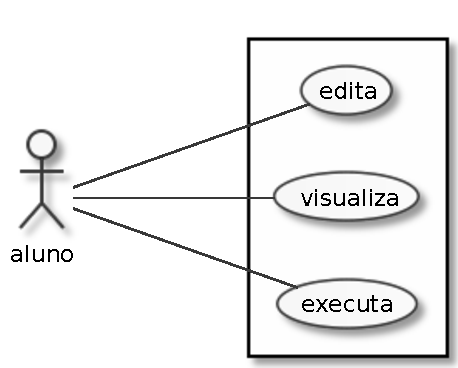
\includegraphics[width=.45\textwidth,height=10cm,keepaspectratio]{figures/caso-de-uso.pdf}
  \caption*{\footnotesize Fonte: Produção do autor, 2016.}
\end{figure}

\subsection{Diagrama de Componentes}

Para o entendimento do processo de funcionamento online na primeira visita e offline por cache nas necessidades posteriores foi desenvolvido o diagrama de componentes que pode ser visto na Figura .
O diagrama de componentes representa, quando implementado, o sistema com seus componentes. Esse diagrama determina a estruturação destes componentes e a interação entre eles, para funcionamento adequado do sistema (GUEDES, 2011). Os componentes do armazenamento local pode ser visto na Figura \ref{fig:componentssw} e na Figura \label{fig:componentsrun} constam os componentes da execução do algoritmo.

\begin{figure}[h]
  \caption{Componentes do processo SW}\label{fig:componentssw}
  \centering
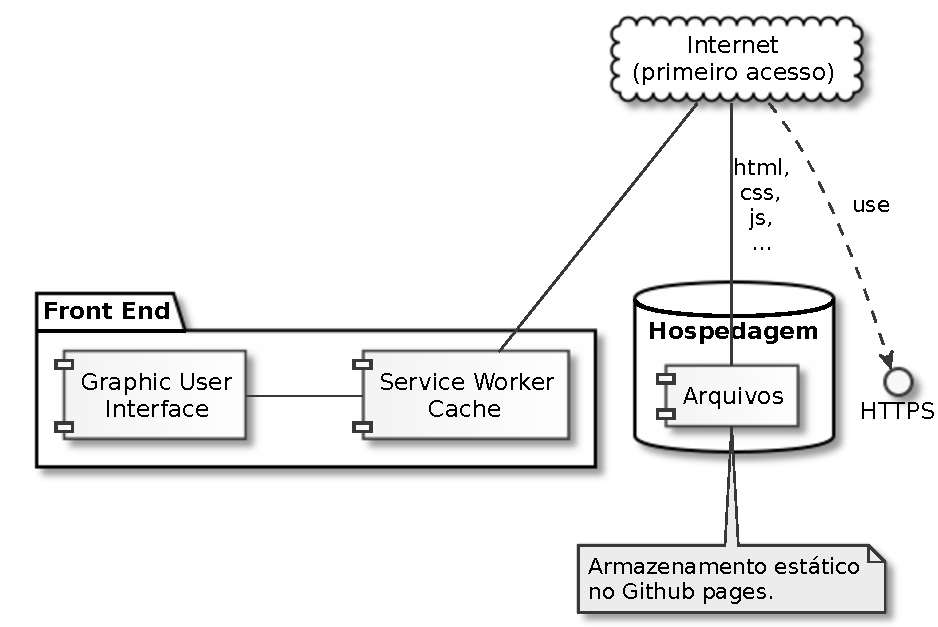
\includegraphics[width=.75\textwidth,keepaspectratio]{figures/components-sw.pdf}
  \caption*{\footnotesize Fonte: Produção do autor, 2016.}
\end{figure}

\begin{figure}[h]
  \caption{Componentes da tradução}\label{fig:componentsrun}
  \centering
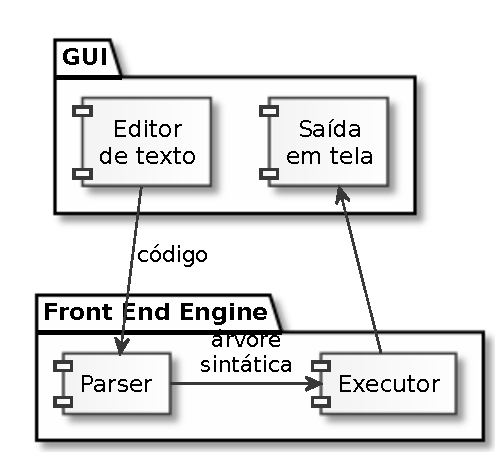
\includegraphics[width=.4\textwidth,keepaspectratio]{figures/components-run.pdf}
  \caption*{\footnotesize Fonte: Produção do autor, 2016.}
\end{figure}

\section{Interface Gráfica}

Como interface gráfica foi mantido o mínimo necessário. Somente o editor de texto e um botão para executar. Foram visualizadas renderizações e tamanhos de telas variados, computadores (Figura \ref{fig:ui-pc}), tablets, smartphones, etc. Seguindo conceitos do Google Material Design foi adicionada uma barra no topo como botão para menu o nome da aplicação, denominada Bizu, e um botão de ação flutuante no canto inferior direito como ícone ``play'' para a execução do algoritmo.

\begin{figure}[h]
  \caption{Interface Desktop}\label{fig:ui-pc}
  \centering
  \setlength{\fboxsep}{0pt}%
\setlength{\fboxrule}{1pt}%
\fbox{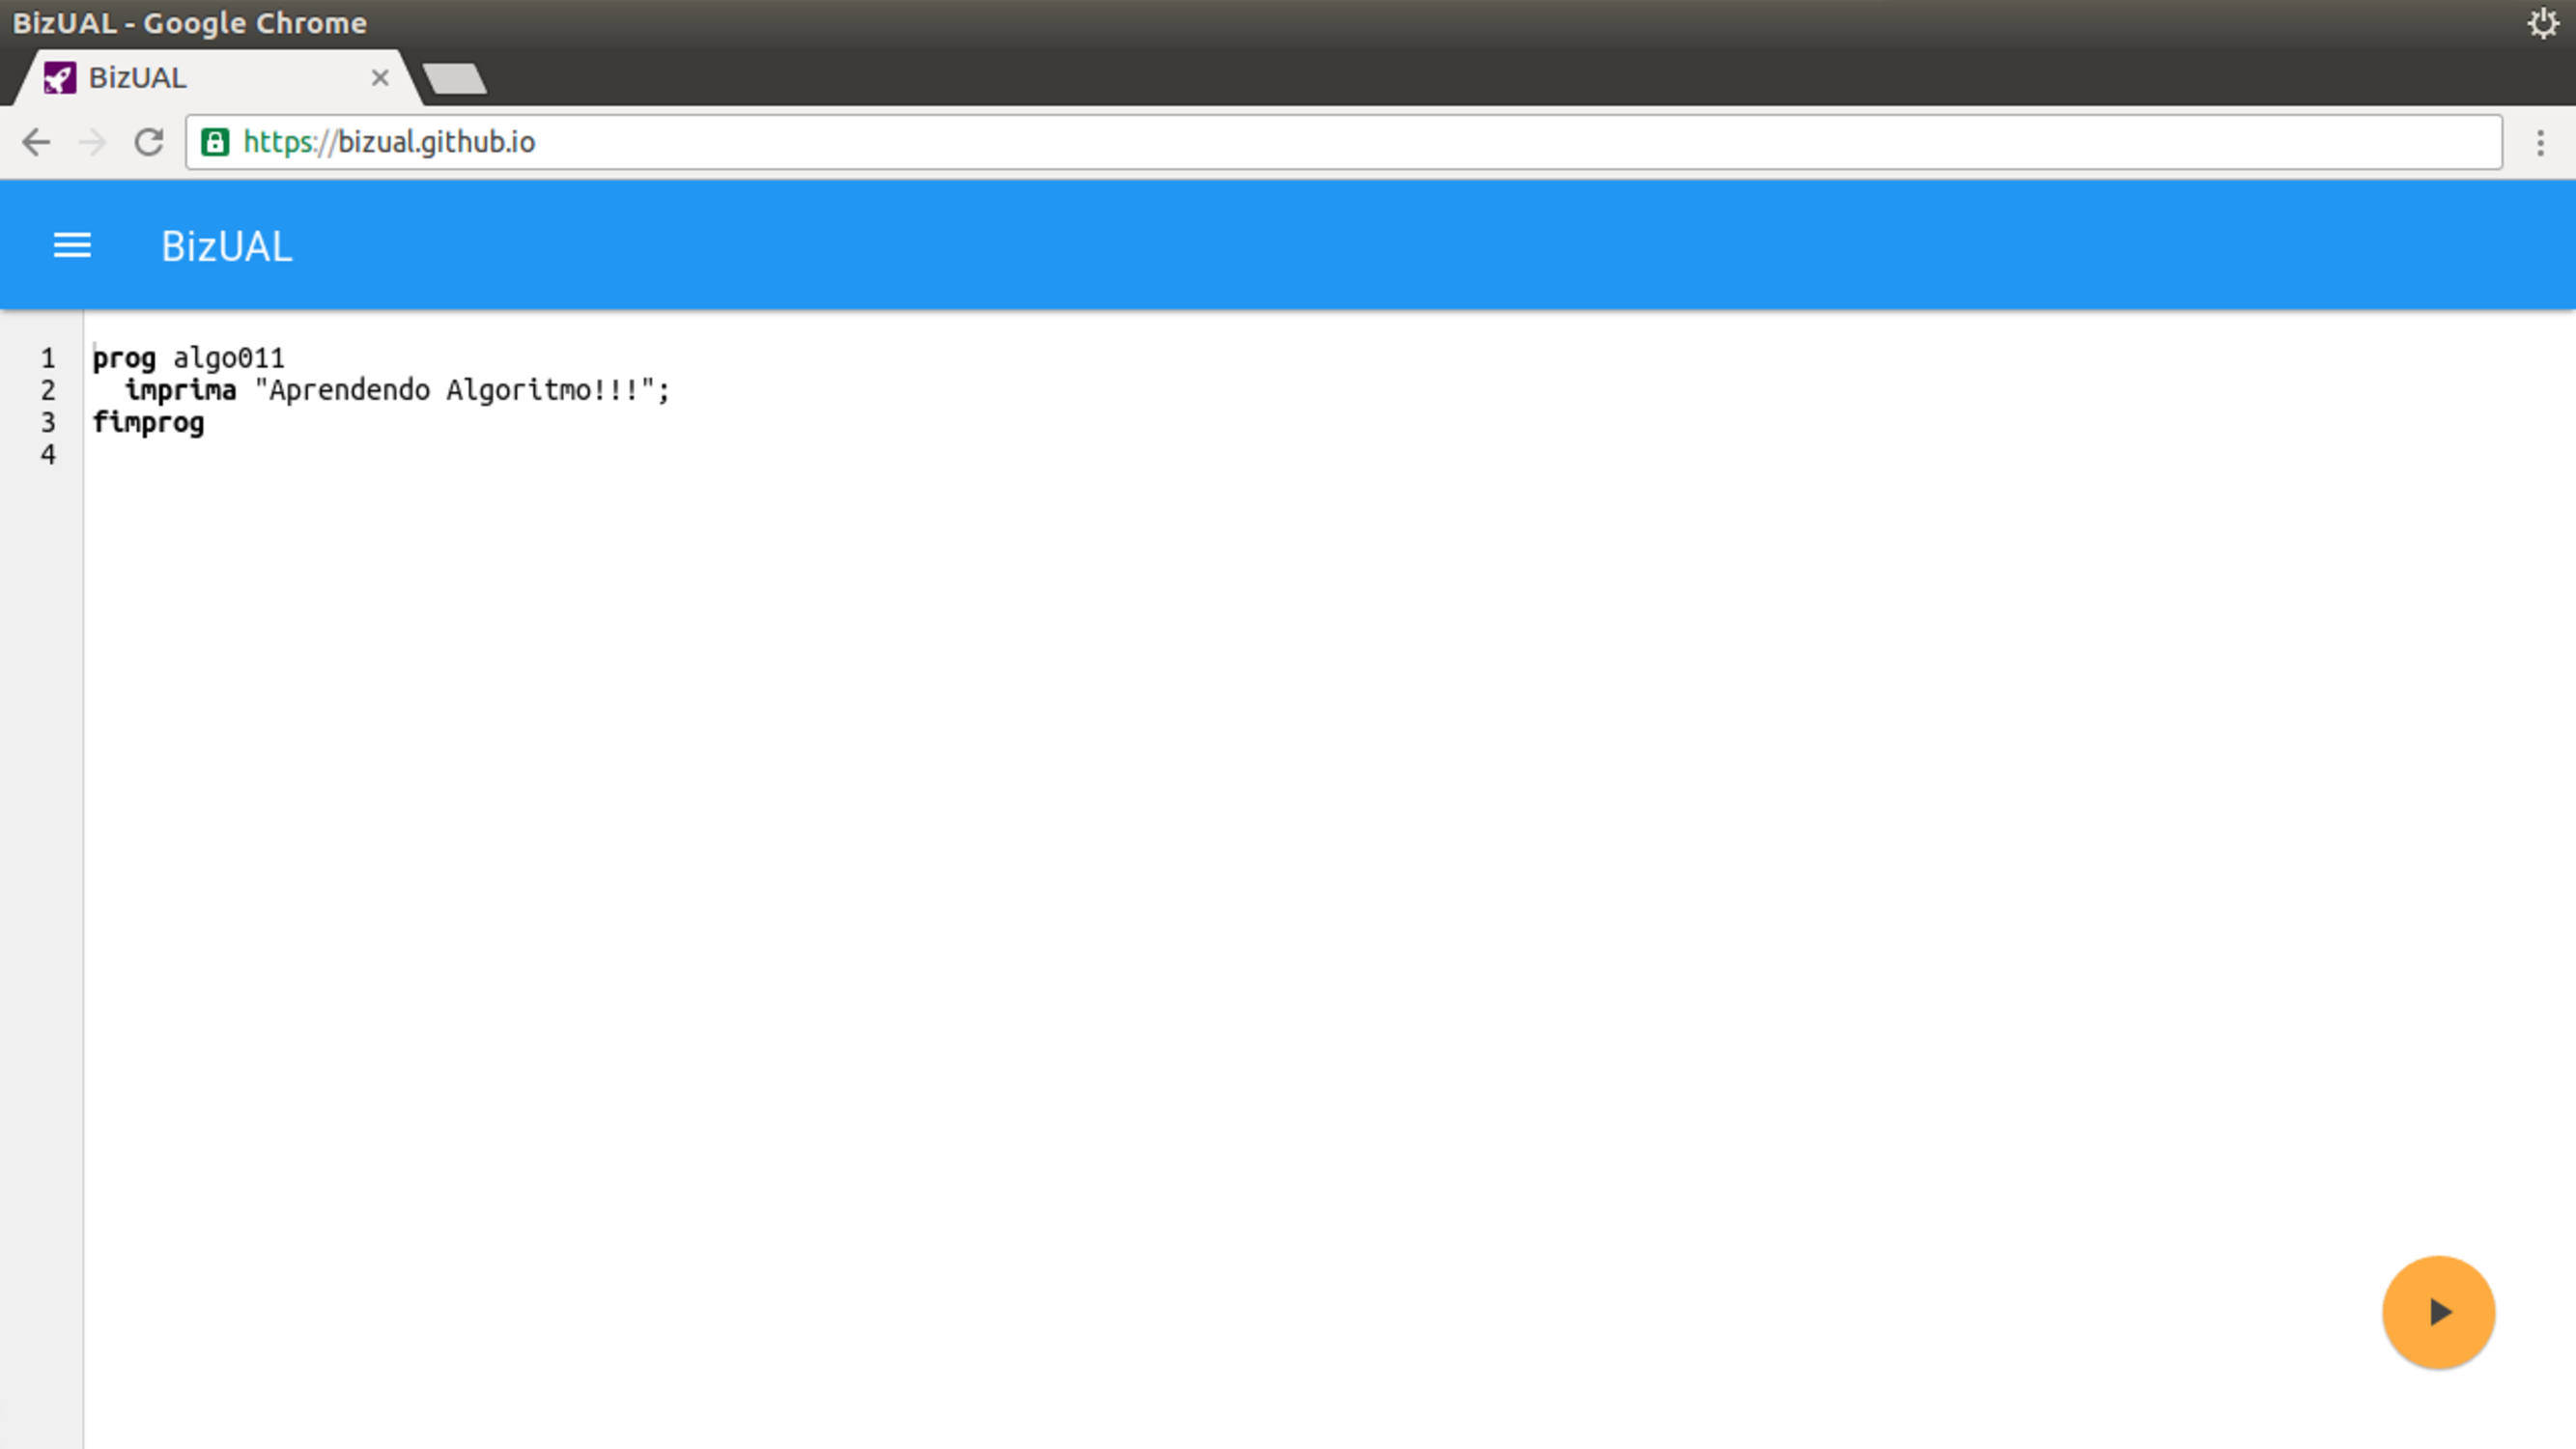
\includegraphics[width=\textwidth,keepaspectratio]{figures/bizual-desktop.pdf}}
  \caption*{\footnotesize Fonte: Produção do autor, 2016.}
\end{figure}

Também na Figura \ref{fig:ui-pc} pode ser notado o nome ``bizUAL'', este foi utilizado para facilitar a identificação do software entre alunos e professores. A escolha do nome surgiu a partir da palavra bizu adicionada a sigla da sintaxe UAL. A gíria \nocite{dicionarioinformal2016}``bizu'' teve origem em quartéis militares, onde os experientes sussurravam dicas para os novatos, os superiores de longe ouviam aquela onomatopéia característica de cochicho ``bzbzbzu'', dando origem ao termo.

%\begin{figure}[h]
%  \caption{Interface Smartphone}\label{fig:ui-phone}
%  \centering
%  \setlength{\fboxsep}{0pt}%
%\setlength{\fboxrule}{1pt}%
%\fbox{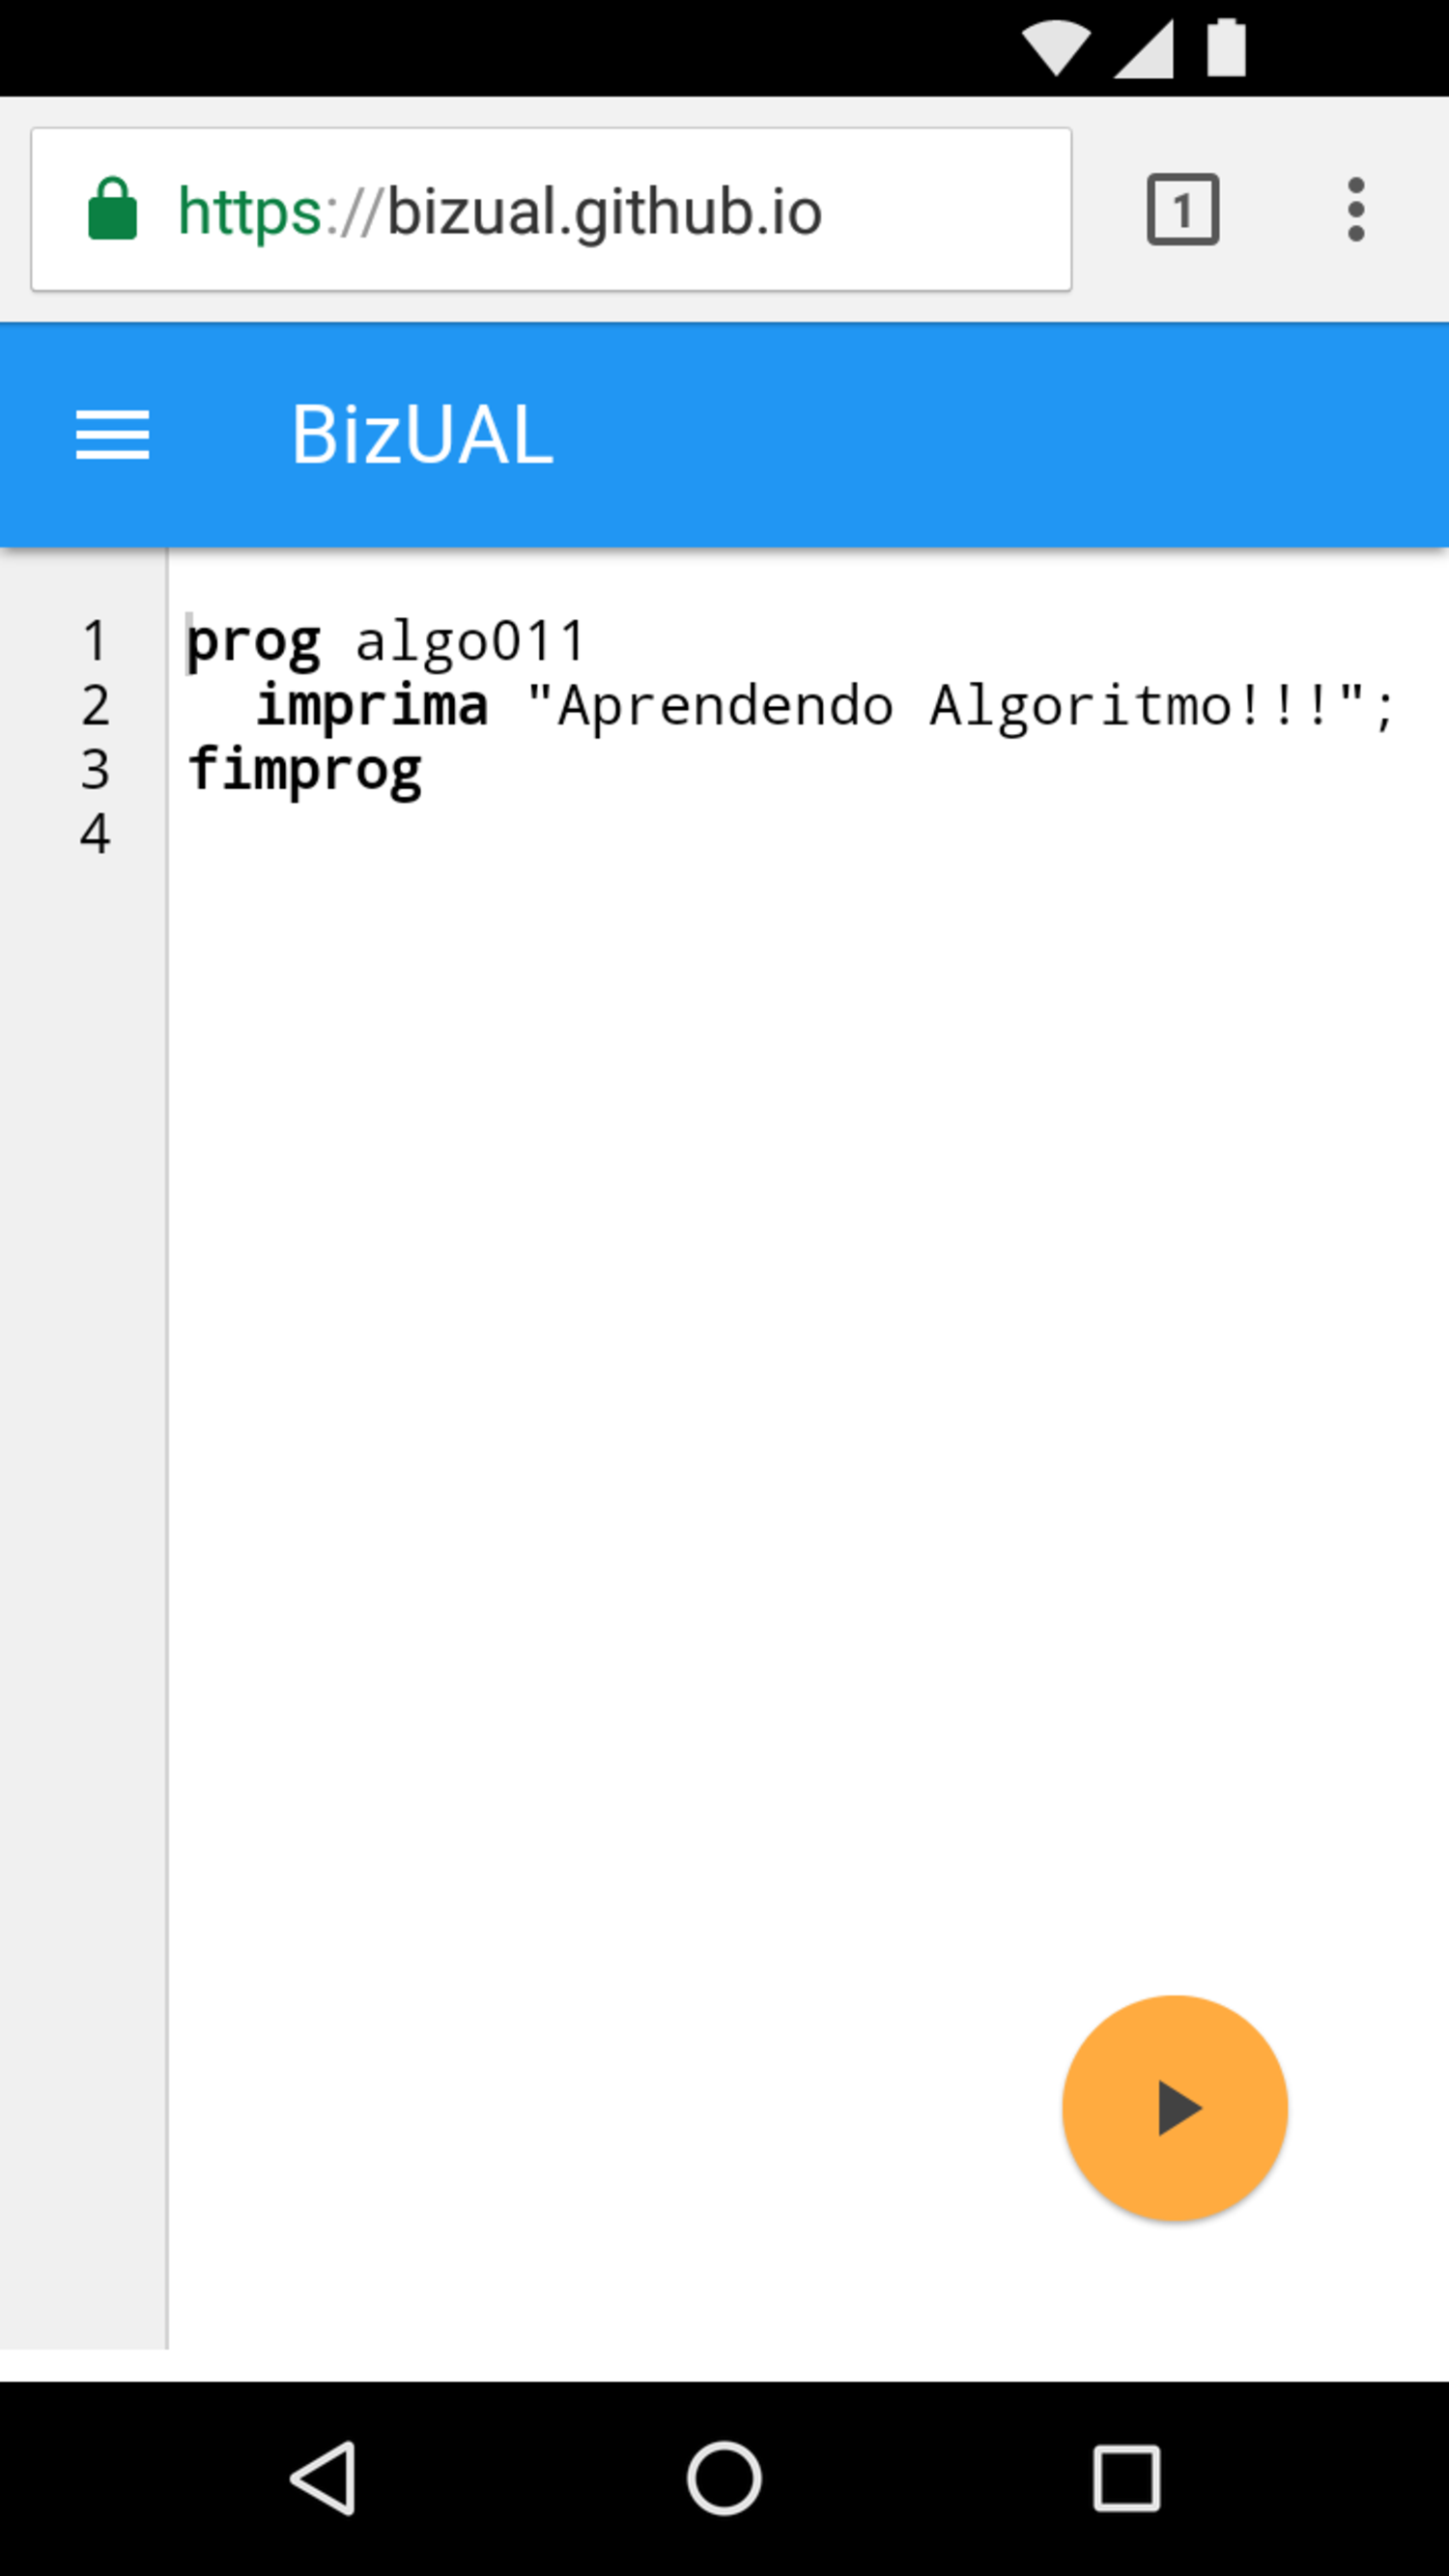
\includegraphics[width=10cm,height=10cm,keepaspectratio]{figures/bizual-smartphone.pdf}}
%  \caption*{\footnotesize Fonte: Produção do autor.}
%\end{figure}

Facilitando a tarefa de construção da interface foi utilizada a biblioteca Material Design Lite (MDL)\nocite{mdl} disponibilizada oficialmente pelo Google. Essa biblioteca possui em seu site uma funcionalidade, na qual cores foram escolhidas.

%Foi utilizada a funcionalidade \textit{Service Worker} a partir de um arquivo manifesto listando o conteúdo que o navegador deve guardar cópia local. Podendo assim ter a internet desconectada após o primeiro acesso que a aplicação continuará acessível.

%Todo o código foi desenvolvido em repositório disponível no github e quando concluído em sua versão mínima movido para seu destino final e podendo ser acessado.\nocite{bizual}

\section{Editor de Código ACE}

%No modelo em que é possível embutir nas páginas web ou aplicações via navegador, já existem editores de código fonte de linguagens de programação. Dentre esses editores de código em texto, os mais utilizados tem-se o ACE\nocite{ace} e o CodeMirror\nocite{codemirror}. Foi optado pelo ACE, pois em análise entendeu-se como sendo mais prático para o uso e criação do modelo da linguagem. A criação do modelo gramatical para destaque da sintaxe, foi considerado como dificuldade relativamente baixa.
No modelo em que é possível embutir nas páginas web ou aplicações via navegador, já existem editores de código fonte de linguagens de programação. Dentre esses editores de código em texto, os mais utilizados tem-se o ACE\nocite{ace} e o CodeMirror\nocite{codemirror}. Foi optado pelo ACE, pela praticidade de sua adição no protótipo e fácil criação do modelo gramatical para destaque de palavras reservadas da linguagem.

Em tecnologia há áreas para experimentações com determinada ferramenta ou tecnologia (\textit{playground}). No caso do editor ACE é disponibilizado uma ``pia de cozinha'' (\textit{Kitchen Sink}\nocite{kitchensink}) conforme Figura \ref{fig:ace-kitchensink}, onde o editor embutido pode ser modificado através de um menu lateral, quanto a linguagem ou tema e outras de suas várias opções.

\begin{figure}[h]
  \caption{Ace \textit{Kitchen Sink}}\label{fig:ace-kitchensink}
  \centering
  \setlength{\fboxsep}{0pt}%
\setlength{\fboxrule}{1pt}%
\fbox{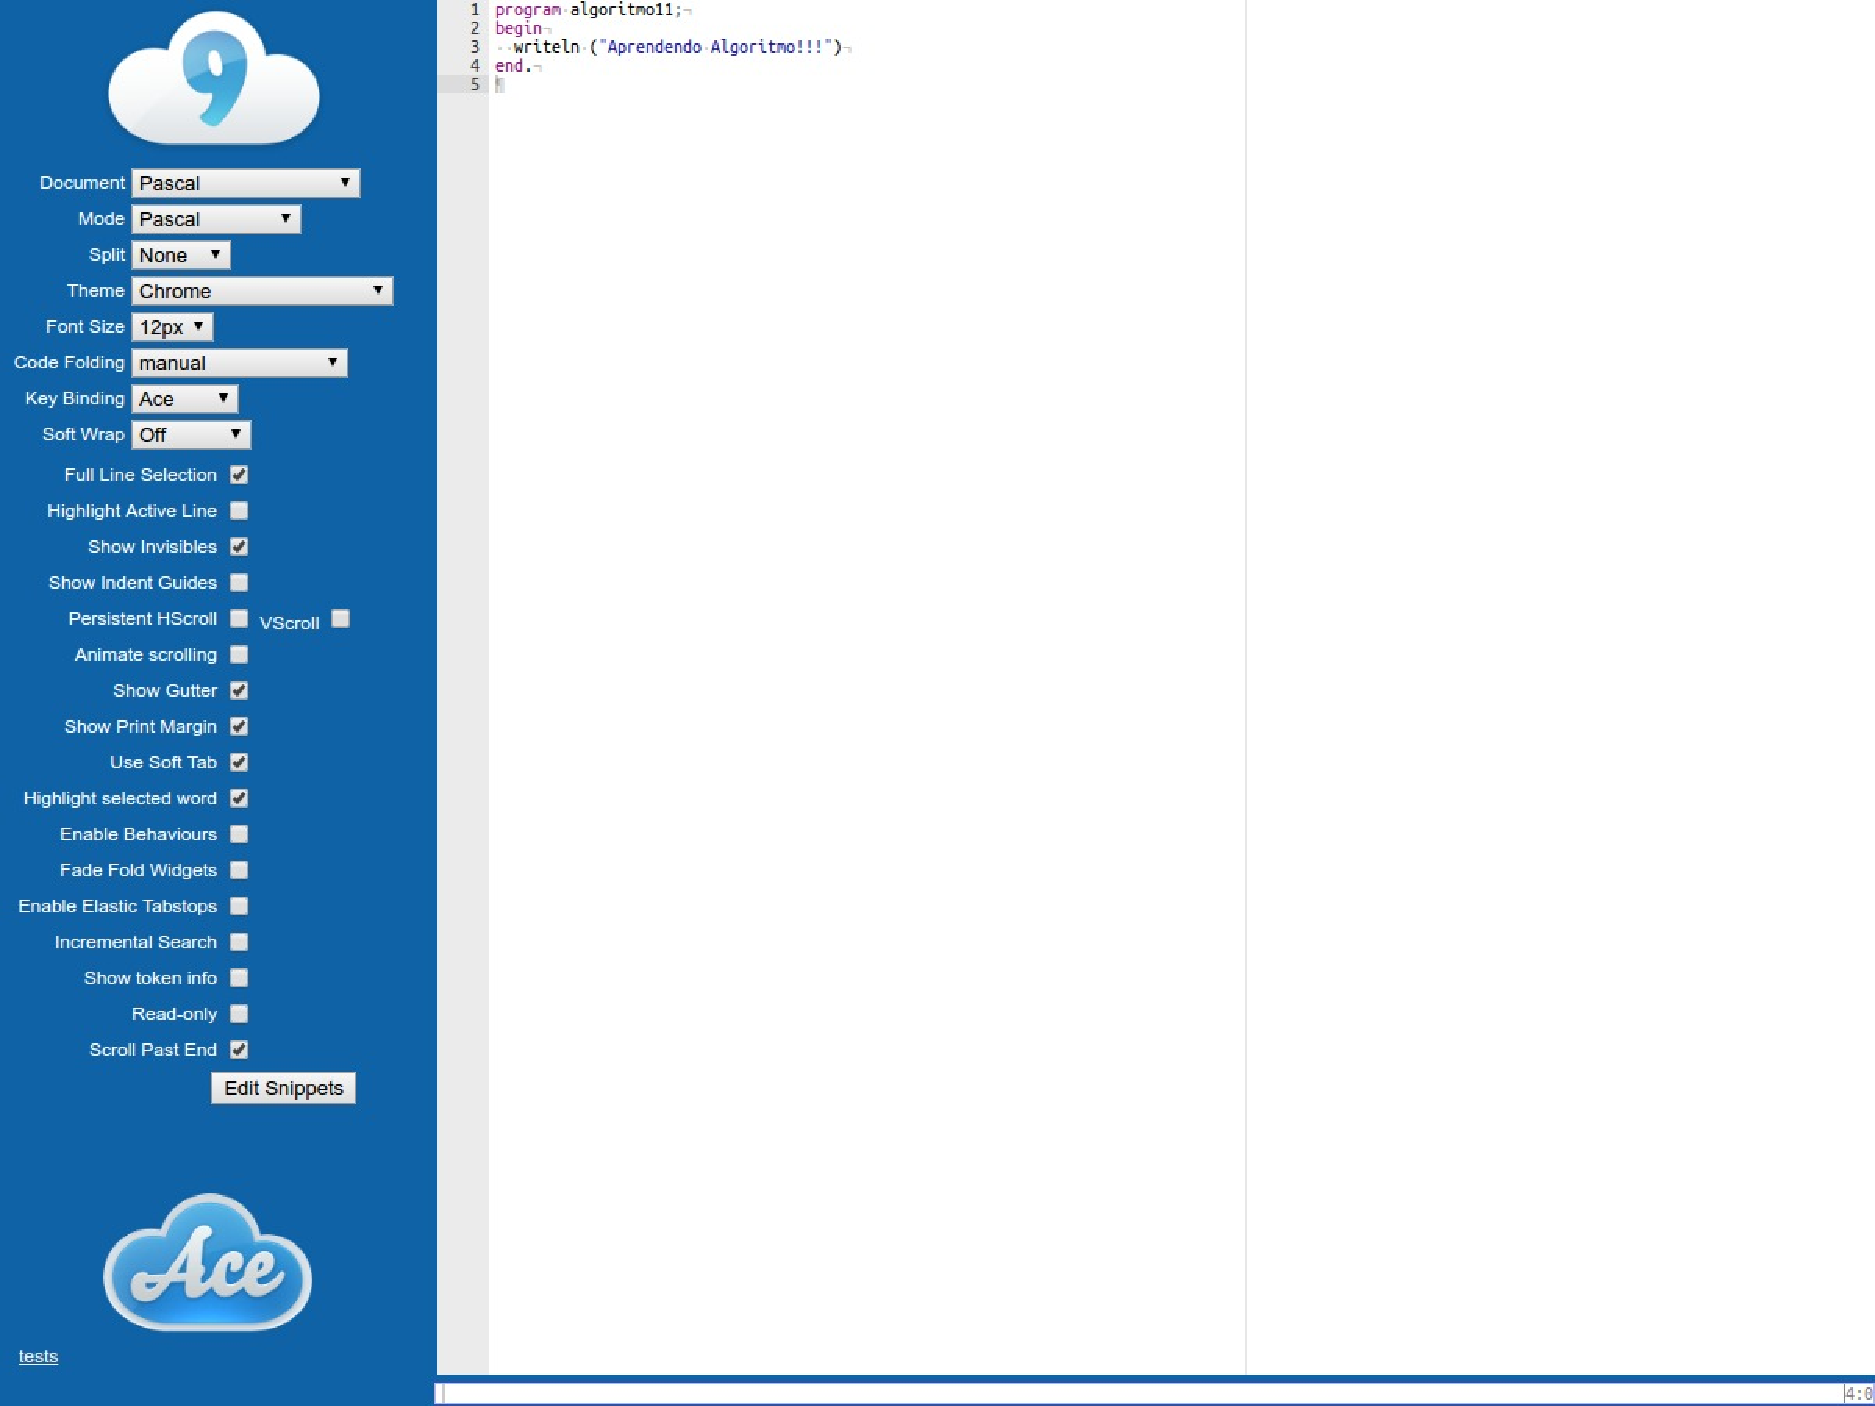
\includegraphics[width=\textwidth,keepaspectratio]{figures/ace-kitchensink.pdf}}
  \caption*{\footnotesize Fonte: Produção do autor, 2016.}
\end{figure}

Inicialmente as funcionalidades pretendidas são todas supridas e outra mais levam a esta ser uma opção útil para evolução da aplicação em trabalhos futuros. Ignorando as duas que dizem respeito ao destacamento de sintaxe em mais de 110 linguagens (customizável, o que permitiu adicionar UAL) e mais de 20 temas (também personalizado para o mesmo estilo encontrado no Editor UAL), as demais funcionalidade estão expostas no Quadro \ref{qua:acefunctions}.

\begin{quadro}[h]
\centering
  \caption{Demais Funcionalidade do Editor ACE}\label{qua:acefunctions}
\begin{tabular}{| l |}\hline
\textbf{Descrição} \\ \hline
Identação automática \\ \hline
Permite documentos com muitas linhas \\ \hline
Atalhos de teclado personalizáveis \\ \hline
Localizar e substituir, podendo utilizar expressões regulares \\ \hline
Alternar entre tabulação suave (espaços) ou tabulação real \\ \hline
Exibir caracteres ocultos \\ \hline
Arrastar e soltar utilizando mouse \\ \hline
Limitação de colunas no texto, com quebra \\ \hline
Retrair ou expantir código \\ \hline
Cursores e seleção múltiplas \\ \hline
Checagem em tempo real para algumas linguagens \\ \hline
Funcionalidade de recortar, copiar e colar \\ \hline
\end{tabular}
  \caption*{\footnotesize Fonte: Produção do autor, 2016.}
\end{quadro}

\section{Módulos para Tradução}

Para resultar na árvore sintática encontrou-se o \textbf{ACORN}\nocite{acorn}, um parser já escrito em JavaScript. A árvore sintática gerada pelo Acorn e representada em JSON está no Quadro \ref{qua:sintaxtree}. Opcionalmente pode ser apresentada, nessa árvore sintática, em cada nó a posição de seu caracter de início e fim.

\begin{quadro}[h]
\centering
  \caption{Árvore sintática gerada pelo Acorn modificado}\label{qua:sintaxtree}
\begin{lstlisting}[style=json,frame=single]
{
  "type": "Program",
  "body": [
    {
      "type": "PrintStatement",
      "print": {
        "type": "CallPrint",
        "arguments": {
          "type": "Literal",
          "value": "Aprendendo Algoritmo!!!",
          "raw": "\"Aprendendo Algoritmo!!!\""
        }
      }
    }
  ],
  "id": {
    "type": "Identifier",
    "name": "algoritmo11"
  }
}
\end{lstlisting}
  \caption*{\footnotesize Fonte: Produção do autor, 2016.}
\end{quadro}

Para a saída, simulando o algoritmo, o \textbf{JS-Interpreter}\nocite{jsinterpreter} foi encontrado como opção. Ele se utiliza do ACORN, recebendo a árvore sintática para poder apresentar a execução de cada instrução.

Tanto no Acorn quanto no JS-Interpreter foi necessário adaptar o código fonte para compreender a estrutura do algoritmo proposto, pois esse foram criados para a própria linguagem em qual foram construídos, Javascript. Foi necessário um processo de engenharia reversa através da reescrita do código para fazer com que eles fossem adaptados ao protótipo. Principalmente devido à não utilização de parênteses para o comando de impressão em tela, diferença que pode ser compreendida no Quadro \ref{qua:comparejsual}.

\lstdefinelanguage{javascript}
{
  morekeywords={
    prog,
    imprima,
    fimprog
  },
  sensitive=true,
  morecomment=[l]{\#},
  morestring=[b]",
}

\begin{quadro}[h]
\centering
  \caption{Diferença de sintaxe Javascript e UAL}\label{qua:comparejsual}
\begin{tabular}{| p{100mm} |}\hline
\multicolumn{1}{|c|}{\textbf{Javascript}} \\ \hline
\begin{lstlisting}[language=javascript,style=table]
document.write("Aprendendo Algoritmo!!!");
\end{lstlisting} \\ \hline
\multicolumn{1}{|c|}{\textbf{UAL}} \\ \hline
\begin{lstlisting}[language=ual,style=table]
imprima "Aprendendo Algoritmo!!!";
\end{lstlisting} \\ \hline
\end{tabular}
  \caption*{\footnotesize Fonte: Produção do autor, 2016.}
\end{quadro}

Em conjunto o Acorn e o JS-Interpreter podem ser vistos na área central da Figura \ref{fig:flux}, funcionando como tradutor para sintaxe UAL resultando na saída em tela simulada, processo indicado como Interpretador. Também é possível verificar na Figura \ref{fig:flux} outros elementos do software: navegador web, editor de texto.

\begin{figure}[h]
  \caption{Esquemático do Interpretador}\label{fig:flux}
  \centering
  \setlength{\fboxsep}{0pt}%
\setlength{\fboxrule}{1pt}%
\fbox{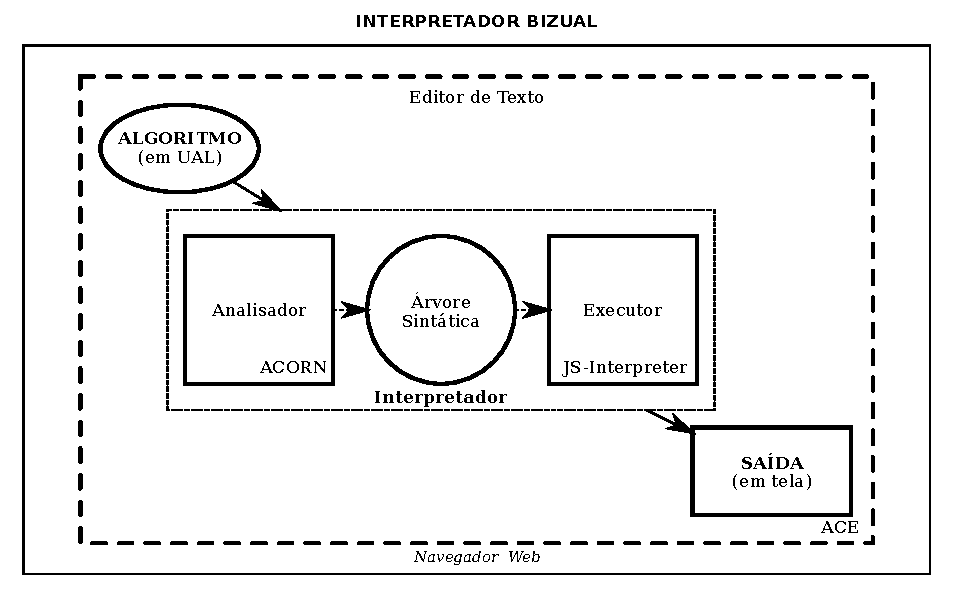
\includegraphics[width=\textwidth,keepaspectratio]{figures/bizual-interpretador.pdf}}
  \caption*{\footnotesize Fonte: Produção do autor, 2016.}
\end{figure}

\section{Acesso \textit{Offline}}

%Ainda não há aderência dentre os desenvolvedores, bem porque ainda não foi finalizada sua especificação. Além de que a primeira tentativa de criar o \textit{AppCache} como solução solução teve um resultado ruim, mas agora com os \textit{Service Workers} a esperança foi renovada.
%
%\subsection{\textit{AppCache}}
%
%Desenvolvido pela consórcio criado para o desenvolvimento do HTML5 veio suprir a necessidade de armazenamento avançado de arquivos utilizados na aplicação web. Sua compatibilidade foi seu adicionada aos navegadores durante sua criação, na tabela \ref{tab:appcache-compatibility}  Porém apesar de simples sua específicação extensa e confusa além de muitas limitações conhecidas levou a criaçao de uma melhor solução. Essa fucionalidade permanece compatível mas é recomendado sua não utilização por motivo da futura remoção dela nos navegadores.

%\begin{table}[h]
%\centering
%  \caption{Suporte à \textit{AppCache} pelos navegadores}\label{tab:appcache-compatibility}
%\begin{tabular}{ C{46pt} | C{46pt} | C{46pt} | C{46pt} | C{46pt} | C{46pt} | C{46pt} }\hline
%IE & Firefox & Safari & Chrome & Opera & iPhone & Android \\ \hline
% & 3.5+ & 4.0+ & 5.0+ & 10.6+ & 2.1+ & 2.0+ \\ \hline
%\end{tabular}
%  \caption*{\footnotesize Fonte: ``Aplicações Web Offline - Dive into HTML5'' por \citeonline{diveintohtml5}.}
%\end{table}
%
%Mesmo tento sido depreciada cabe, até por comparação, explicar seu funcionamento. Ela utiliza, como explica \citeonline{diveintohtml5}, apenas um arquivo de texto onde lista todos os arquivos de imagem, estilização, scripts de programação, entre outros (ver quadro \ref{qua:html-root}). Esse arquivo declarado manifesto deve ser desclarado como atributo no etiqueta de abertura do html (veja quadro  \ref{qua:cache-appcache}).
%
%\let\origthelstnumber\thelstnumber
%\makeatletter
%\newcommand*\Suppressnumber{%
%  \lst@AddToHook{OnNewLine}{%
%    \let\thelstnumber\relax%
%     \advance\c@lstnumber-\@ne\relax%
%    }%
%}
%
%\newcommand*\Reactivatenumber[1]{%
%  \lst@AddToHook{OnNewLine}{%
%   \let\thelstnumber\origthelstnumber%
%   \setcounter{lstnumber}{\numexpr#1-1\relax}%
%   %\advance\c@lstnumber\@ne\relax%
%  }%
%}
%
%\makeatother
%
%\begin{quadro}[h]
%\centering
%  \caption{Código HTML ignorando cabeçalho e corpo}\label{qua:html-root}
%\begin{lstlisting}[numbers=left,escapeinside=\$\$,frame=single]
%<!DOCTYPE html>
%<html lang="pt-BR" manifest="cache.appcache">
%  <head>$\Suppressnumber$
%    (...)$\Reactivatenumber{16}$
%  </head>$\Reactivatenumber{17}$
%  <body>$\Suppressnumber$
%    (...)
%  </body>$\Reactivatenumber{51}$
%</html>
%
%\end{lstlisting}
%  \caption*{\footnotesize Fonte: Produção do autor.}
%\end{quadro}
%
%\begin{quadro}[h]
%\centering
%  \caption{Arquivo de manifesto \textit{appcache}}\label{qua:cache-appcache}
%\begin{lstlisting}[numbers=left,frame=single]
%CACHE MANIFEST
%
%# Updated: 2016-11-90T01:27:00-02:00
%
%# Main page
%
%# CSS
%style/material.blue-orange.min.css
%style/main.css
%
%# Fonts
%style/fonts/material-icons.css
%style/fonts/MaterialIcons-Regular.eot
%style/fonts/MaterialIcons-Regular.woff
%style/fonts/MaterialIcons-Regular.woff2
%style/fonts/MaterialIcons-Regular.ttf
%
%# Other resources
%
%# JavaScript
%js/material.min.js
%js/aceual.js
%
%favicon.ico
%
%NETWORK:
%*
%
%\end{lstlisting}
%  \caption*{\footnotesize Fonte: Produção do autor.}
%\end{quadro}

Com auxílio de \textbf{\textit{Service Workers}} (SW) é possível resolver a navegação \textit{offline}. Está sendo desenvolvido, como explica \citeonline{swfirstdraft}, por um esforço colaborativo entre grandes empresas como Google, Mozilla e outras, sua implementação tem sido constante principalmente nos navegadores Chrome e Firefox. Realmente estimulante para os interessados na competição entre \textit{web} e aplicações nativas nos sistemas operacionais.

Sua implementação no modo mais básico em uma aplicação de página única pode ser considerada simples. Porém sua versatilidade e aplicabilidade é incrivelmente mais extensa. Inicialmente é necessário informar ao navegador o arquivo Javascript que será o controlador, este arquivo se comporta como um \textit{proxy} local. Para indicar o arquivo ao navegador utiliza-se o comando de registro (presente no Quadro \ref{qua:swregister}), após testar se há compatibilidade.

\lstdefinestyle{swreg}
{
  morestring  = [s]{<script}{script>},
  basicstyle  = \small\ttfamily\color{darkgrey},
  stringstyle = \bfseries\color{black},
}

\begin{quadro}[h]
\centering
  \caption{HTML destacando o registro do SW}\label{qua:swregister}
\begin{lstlisting}[style=swreg,frame=single]
<!DOCTYPE html>
<html>
  <head>
    (...)
  <body>
    (...)a
    <script>
      if (navigator.serviceWorker !== undefined) { navigator.serviceWorker.register('sw.js'); }
    </script>
</html>

\end{lstlisting}
  \caption*{\footnotesize Fonte: Produção do autor, 2016.}
\end{quadro}

Dentro do arquivo \texttt{sw.js}, notável em Quadro \ref{qua:swjs}, constam três eventos: um de instalação para quando o navegador realiza a instalação (\textbf{\textit{install}}) de acordo com o registro, um quando ativar (\textbf{\textit{activate}}) o serviço e outro para captura de ação de rede (\textbf{\textit{fetch}}), onde iria naturalmente requisitar determinado recurso. O evento de instalação lista os arquivos a serem armazenados e o de rede manipula a utilização os arquivos armazenados.
%
%\lstdefinestyle{swjs}
%{
%  morestring  = [s]{`use}{strict';},
%  stringstyle = \color{darkgrey},
%  keywordstyle = \color{darkgrey},
%  commentstyle = \color{darkgrey},
%  morecomment  = [l]{/*},
%}
%style=swjs,
\begin{quadro}[h]
\centering
  \caption{Conteúdo do arquivo SW}\label{qua:swjs}
\begin{lstlisting}[frame=single]
var cacheFiles = [`./', 'css/all.css', 'js/page.js', 'js/material.min.js', 'js/aceual.js', 'js/parser.js', 'js/intepreter.js', 'imgs/icon.png'];
self.oninstall = function (event) {
  event.waitUntil(caches.open(`bizual-static-v1').then(function (cache) { return cache.addAll(cacheFiles); }));
};
self.onactivate = function (event) {
  event.waitUntil(caches.keys().then(function (keys) { return Promise.all(keys.map(function (key) { if (key !== cacheName) { return caches.delete(key); } })); }));
};
self.onfetch = function (event) {
  event.respondWith(caches.match(event.request));
};
\end{lstlisting}
  \caption*{\footnotesize Fonte: Produção do autor.}
\end{quadro}

Durante o trabalho tem sido utilizada a denominação ``navegador moderno'', para nosso estudo são navegadores que apostam em novas tecnologia que estejam surgindo. Normalmente podem ser considerados o Google Chrome, Mozilla Firefox e Opera. A Microsoft vêm flexibilizando essas adoções nas últimas versões e do seu substituto o Edge, porém quando tecnologias ainda em rascunho ela opta por sua definição e maturidade. A Tabela \ref{tab:swcompatibility} apresenta como está, mesmo que parcial, essa compatibilidade. Ressaltando o quão recente é essa adoção, as versões lançadas somente neste ano como estáveis entre 9 de setembro e 23 de outubro, são nesses navegadores a primeira implementação ocorrida. Apenas o Google Chrome para desktop possui compatibilidade nas versões anteriores, desde 2 de maio também de 2016.

\begin{table}[h]
\centering
  \caption{Suporte à SW pelos navegadores}\label{tab:swcompatibility}
\begin{tabular}{ C{46pt} | C{46pt} | C{46pt} | C{46pt} | C{46pt} | C{46pt} | C{46pt} }\hline
Edge & Firefox & Chrome & Safari & Opera & iOS & Android \\ \hline
 & 49+ & 49+ &  & 41+ &  & 5.0+ \\ \hline
\end{tabular}
  \caption*{\footnotesize Fonte: Produção do autor, baseado em \citeonline{swcaniuse}.}
\end{table}

Algumas observações são necessárias sobre a Tabela \ref{tab:swcompatibility}, o Microsoft \textbf{Edge} está nessa compatibilidade como ``em desenvolvimento'', e o Internet Explorer (IE) foi intencionalmente ignorado por certamente nunca receber essa implementação já que seu desenvolvimento foi descontinuado em favor do Edge. O \textbf{Safari} da Apple utiliza motor Webkit e ele está com a situação, quanto essa compatibilidade, como ``sob consideração''. E o \textbf{Android} 4.4.4 já utilizava WebView do Chrome mas só na 5.0 veio nativa e independente, porém instalar a última versão do Google Chrome para esse sistema operacional \textit{mobile} tem o mesmo efeito, desde WebView ou o navegador Google Chrome para Android na versão 53.

\ifdraft{}{
%\section{Ferramentas Utilizadas}

%
%
%\section{Processo Criacional}
%
%\subsection{Git e Github}
%
%\subsection{Node.js e Grunt}
%
%\subsection{SASS}
%
%\subsection{TDD}
%
%\subsection{\textit{Material Design}}
%
%\subsubsection{MDL}
%
%\subsection{Inspirações}
}
